\section{Steering}\label{sec:steering}

Another major component of a navigation subsystem is the path execution componenet. There are a number of parts that make up a path execution component; in this thesis, there are three such compenents: steering, trajectory generation and path planning. The lowest-level component is steering. Steering's task is to take a desired robot state (this represents the ideal state of the robot at a given time) and the current robot state and, from those two inputs, produce a set of commands that will make the robot's current state converge on the desired state. The state of the robot is not simple a position and orientation, but also includes parameters such as translational and angular velocities and curvature.

\subsection{State Description}\label{subsec:steering_state}

In the precision steering algorithms developed for this thesis, the final version of the state description was made up of the fields described in \autoref{table:desired_state_description}.

\begin{table}[htbp]
	\begin{tabularx}{\textwidth}{|r|X|}
		\hline
		Name & Description \\
		\hline
		header & This is a standard ROS header type that contains information such as the state's timestamp as well as what reference frame the desired pose is in. \\
		\hline
		segment\_type & An integer enum representing the type of segment that generated this desired state, such as a straight line segment, constant curvature arc segment or spin-in-place segment. \\
		\hline
		segment\_number & The ID number of the segment that generated this state. \\
		\hline
		pose & A six degree of freedom pose, containing x, y and z coordinates as well as roll, pitch and yaw angles. \\
		\hline
		speed & The desired speed for this state. Whether the speed is in meters per second or radians per second depends on the \emph{segment\_type}. \\
		\hline
		rho & The desired curvature for this state. Not used for spin-in-place segments. \\
		\hline
		segment\_distance & How far along the path segment this state corresponds to. \\
		\hline
	\end{tabularx}
	\caption{Steering Desired State Field Description \label{table:desired_state_description}}
\end{table}

Of the fields listed in \autoref{table:desired_state_description}, most of the fields listed are obvious choices for inclusion in the state. For example, if part of the steering algorithm's task is to move the robot to a certain position and orientation in the environment, then obviously the steering algorithm needs that pose in order to move the robot to it. Other fields in this parameterization of the desired state are mainly for informational purposes or consistency with the structures used by the trajectory generator, such as the segment number or segment distance, and were not used by the steering algorithms themselves. One important choice is the parameterization of the segment type field used in this final version.

Originally, only two segment types were used: line segments and constant curvature arc segments. For the steering algorithms, there was no difference in interpretation of those two segment types. While these worked well for most path segments, representation of spin-in-place segments was somewhat hacky, simplying representing them as arcs with very small radii (e.g. less than 1 $\mu m$). Such a representation was acceptable at a theoretical level, as arcs with very small radii are reasonable approximations of a spin-in-place, but led to numerical stability issues when using such small numbers in the steering algortihms due to floating point math behavior on modern computers. In order to solve those numerical stability issues, a third segment type was introduced: the spin-in-place segment. These segments were assumed to have no translational offset and changed the interpretation of the desired speed from a translational speed to a rotational speed.

\subsection{Steering Algorithms}\label{subsec:steering_algorithms}

Two different steering algorithms were developed and evaluated for use in this precision navigation system. The first of these is an algorithm called \emph{second-order steering} (see \autoref{subsubsec:second_order_steering} \todo{fix the reference name to subsubsection}) and the second, developed to address deficiencies in the first, is called \emph{phase space steering} (see \autoref{subsubsec:phase_space_steering}). Both of these algorithms have the same form, as laid out in \autoref{alg:generic_steering_algorithm}.

\begin{algorithm}
\caption{Generic Steering Algorithm}
\label{alg:generic_steering_algorithm}
\DontPrintSemicolon

\KwIn{$\hat{x_t}$, $x_t$}
\KwOut{$v$, $\omega$}

$v$, $\omega$ = executeSteeringAlgorithm($\hat{x_t}$, $x_t$)\;

\end{algorithm}

The inputs to \autoref{alg:generic_steering_algorithm} are the desired robot state ($\hat{x_t}$) and the current robot state ($x_t$) as estimated by the precision localization system. The steering algorithm outputs are the translational velocity ($v$) and rotational velocity ($\omega$) that, when commanded to the robot base, are the best commands to ensure convergence to the desired state. Since these are only individual commands, not a sequence of them, the steering algorithm must be run at a regular rate, recomputing the commands each time, to ensure convergence. In this thesis, the steering algorithms were tuned to run at 20 Hz.

Both steering algorithms use the same equation to determine the output speed command, $v$. \eqref{eq:steering_v_lfollow} gives this equation.

\begin{equation}
v = v_{des} + k_v \cdot Lfollow
\label{eq:steering_v_lfollow}
\end{equation}

In \eqref{eq:steering_v_lfollow}, $v$ is the output desired velocity, $v_{des}$ is the desired velocity according to the input desired robot state and $k_v$ is a tunable gain constant. $Lfollow$ is the error between the robot's state and the desired state along the desired path. $Lfollow$ represents how far in front or behind the robot is from the desired state and, accordingly, modifies the desired velocity to correct this error along the desired path. For example, if the robot has fallen ``behind'' the desired state, the output velocity is increased such that it can reduce the tangential error (and hence $Lfollow$ term). See \autoref{subsec:lfollow_discussion_steering} \todo{fix subsection naming} for more discussion of the $Lfollow$ term.

\subsubsection{Second-Order Steering}\label{subsubsec:second_order_steering}

The initial steering algortihm used in this thesis is called \emph{second-order steering}. This algorithm implements \eqref{eq:steering_v_lfollow} and \eqref{eq:second_order_steering_omega}.

\begin{equation}
\omega_{cmd} = v \cdot \left(k_d \cdot d + k_{\Psi} \cdot \delta\Psi + \rho_{des}\right)
\label{eq:second_order_steering_omega}
\end{equation}

In \eqref{eq:second_order_steering_omega}, $\omega_{cmd}$ is the output rotational velocity, $v$ is the output of \eqref{eq:steering_v_lfollow}, $\rho_{des}$ is the curvature from the desired state and $k_d$ and $k_{\Psi}$ are tunable gains. $\delta\Psi$ is the difference between the orientation of the desired state and the robot's current state (constrained to the interval $\left[-\pi,\pi\right]$). $d$ is the perpendicular offset of the robot's position from the desired state and represents how far ``off'' the desired path the robot is. Note that $d$ is calculated relative to the desired state extended along its tangent vector in both directions and not necessarily just the desired state's \emph{pose} member described in \autoref{table:desired_state_description}. 

\begin{figure}
\centering
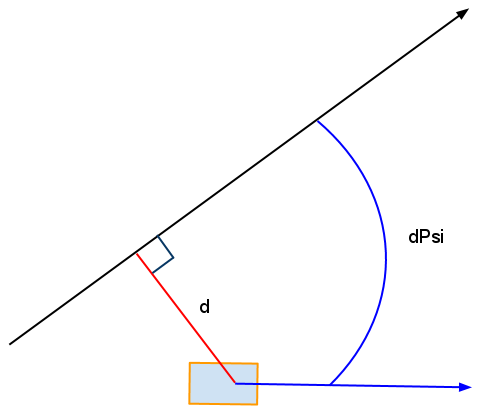
\includegraphics[width=0.75\textwidth]{images/steering_drawing}
\caption{Steering Variable Diagram \label{fig:steering_drawing}}
\end{figure}

\autoref{fig:steering_drawing} is a graphical representation of $d$ and $\delta\Psi$ for a sample robot state and desired state. The black arrow in \autoref{fig:steering_drawing} is the desired state extended along its tangent vector in both directions, the rectangle with orange outline is the robot's current footprint, the blue arrow represents the robot's current position (base of the arrow) and heading (direction of arrow). $d$ in \autoref{fig:steering_drawing} is the $d$ term described above and used in \eqref{eq:second_order_steering_omega}. $dPsi$ in \autoref{fig:steering_drawing} is the $\delta\Psi$ term described above and used in \eqref{eq:second_order_steering_omega}.

While \emph{second-order steering} is a straightforward control algorithm both theoretically and in implementation, it does have some significant drawbacks for precision navigation on an indoor mobile robot. The most significant drawback is that the attraction region \todo{better name for this than ``attraction region''?} of the controller (the contour in control space where the controller will converge to zero error) varies strongly with $k_d$ and $d$. When either of those values is too large, \eqref{eq:second_order_steering_omega} will be dominated by the $k_d \cdot d$ term and lead to very high rate rotational velocity commands. Because of their large magnitude, these commands will basically cause the robot to spin-in-place extremely fast or do large loops far from the desired state; either of these behaviors will not lead to convergence. For precision navigation, the steering algorithm should converge quickly to the desired path, necessitating larger values of $k_d$, but the larger the $k_d$ used, the less lateral offset $d$ required to put \emph{second-order steering} outside of its region of attraction.

Solving this problem required a re-exaxmination of the \emph{second-order steering} algorithm. Specifically, there are two error terms used in \eqref{eq:second_order_steering_omega}: $k_d \cdot d$ and $k_{\Psi} \cdot \delta\Psi$. The $k_{\Psi} \cdot \delta\Psi$ term, which zeroes out error between the desired state's orientation and the robot's current orientation, is relatively stable because the error between desired orientation and actual robot orientation, $\delta\Psi$, is bounded to the interval $\left[-\pi,\pi\right]$. Because of that bounding constraint, $k_{\Psi}$ can be tuned relative to that interval to be both aggressive in converging to zero orientation error while not having a detrimental effect on the controller's attraction region. The other error term in \eqref{eq:second_order_steering_omega}, $k_d \cdot d$, zeroes out lateral offset error between the desired state and the robot's current state. In effect, it produces a desired heading error between the robot's current orientation and the desired state's orientation such that the robot will move towards the desired state and not simply along the desired state's orientation. This insight led the second steering algorithm developed for this thesis, \emph{phase space steering} (see \autoref{subsubsec:phase_space_steering}).

\subsubsection{Phase Space Steering}\label{subsubsec:phase_space_steering}

The second, improved steering algortihm used in this thesis is called \emph{phase space steering}. This algorithm implements \eqref{eq:steering_v_lfollow} and \eqref{eq:phase_space_steering_omega}.

\begin{equation}
\omega_{cmd} = k_\Psi \cdot \left( \delta\Psi - f\left( d \right) \right) + v * \rho_{des}
\label{eq:phase_space_steering_omega}
\end{equation}

In \eqref{eq:phase_space_steering_omega}, $\omega_{cmd}$ is the output rotational velocity, $v$ is the output of \eqref{eq:steering_v_lfollow}, $\rho_{des}$ is the curvature from the desired state and $k_{\Psi}$ is a tunable gain. $\delta\Psi$ and $d$ have have the same meaning as previously described in \autoref{subsubsec:second_order_steering} and shown in \autoref{fig:steering_drawing}, with $\delta\Psi$ constrained to the interval $\left[-\pi,\pi\right]$. The key difference between \eqref{eq:second_order_steering_omega} and \eqref{eq:phase_space_steering_omega} is in the treatment of the lateral offset $d$. In \eqref{eq:phase_space_steering_omega}, $f$ is a non-linear mapping function that maps a given lateral offset $d$ to a desired $\delta\Psi$, such that that desired $\delta\Psi$ would cause the robot to head back towards the desired state and reduce the lateral offset $d$. The particular non-linear mapping function used in this thesis is a simple piecewise linear function, shown in \autoref{fig:phase_space_linear_function_graph} and given in \eqref{eq:phase_space_steering_linear_function}.

\begin{equation}
f\left( d \right) =
	\begin{cases}
		-\pi/2 & \text{if } s \cdot d < -\pi/2 \\
		s \cdot d & \text{if } -\pi/2 \leq s \cdot d \leq \pi/2 \\
		\pi/2 & \text{if } s \cdot d > \pi/2
	\end{cases}
	\label{eq:phase_space_steering_linear_function}
\end{equation}

In \eqref{eq:phase_space_steering_linear_function}, $d$ is the lateral offset that needs to be mapped to a desired $\delta\Psi$. $s$ is the slope of the line used and is the only tunable parameter of this mapping function. The output is bounded to the interval $\left[-\pi/2,\pi/2\right]$ as, for any robot orientation and lateral offset, no more than a ninety degree rotation is required to point the robot towards the desired state. Limiting the output to that interval also prevents arbitrarily large lateral offsets from removing the controller from its attraction region. For any $d$ and $\delta\Psi$, a properly tuned \emph{phase space steering} controller will eventually converge to the desired state vector given enough obstacle-free space.

\begin{figure}[htbp]
\centering
\subfloat[Linear Function]{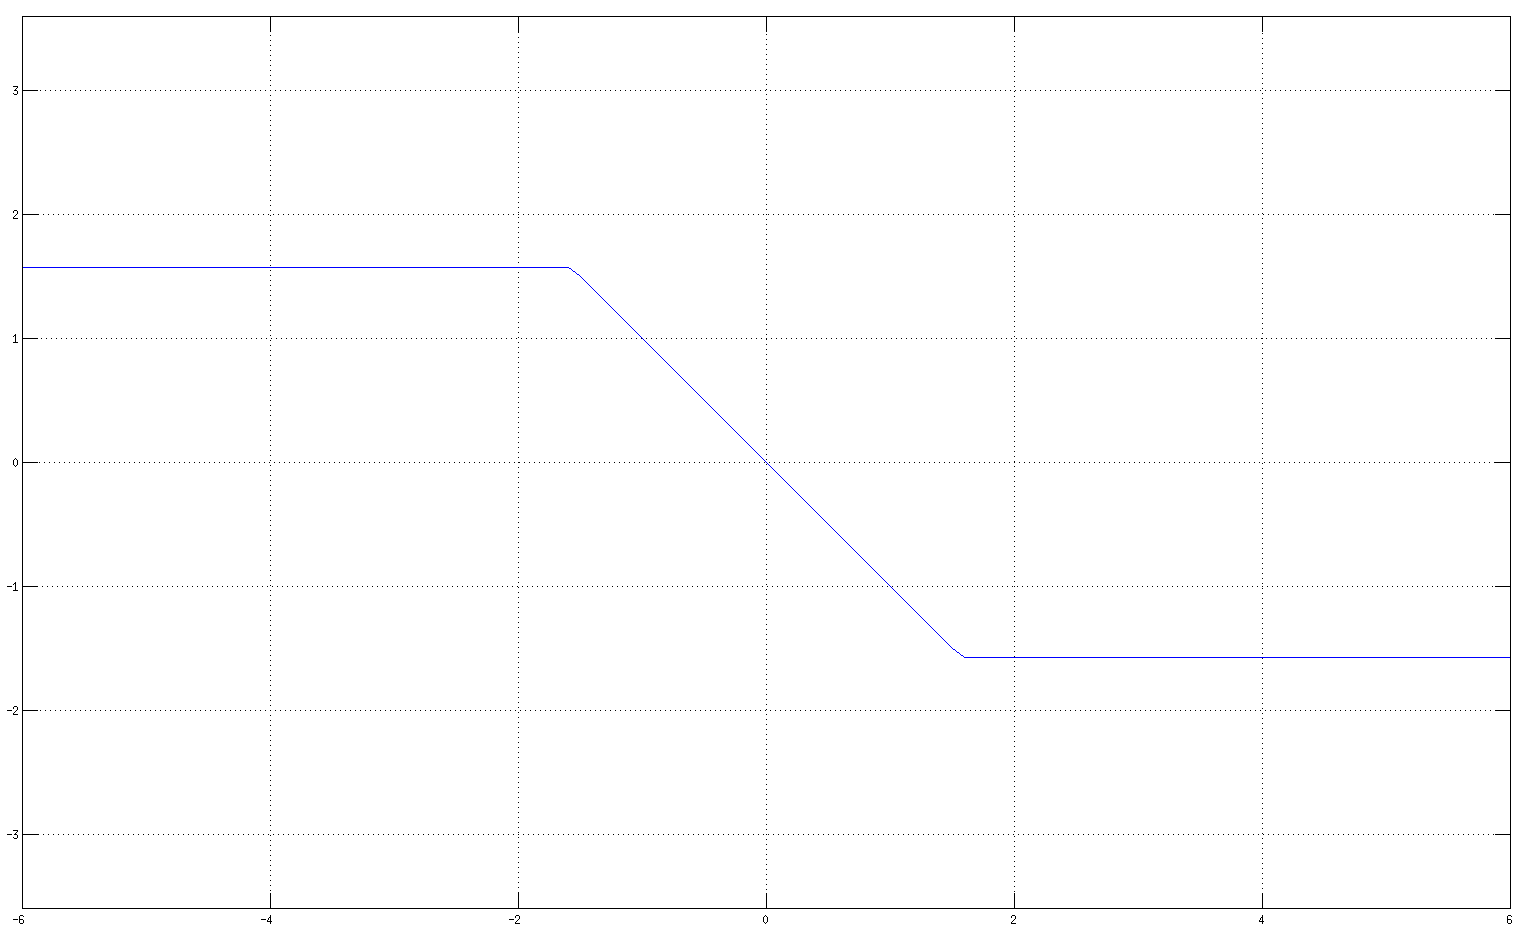
\includegraphics[width=0.5\textwidth]{images/phase_space_linear_function_graph}\label{fig:phase_space_linear_function_graph}}
\hfill
\subfloat[Hyperbolic Tangent Function]{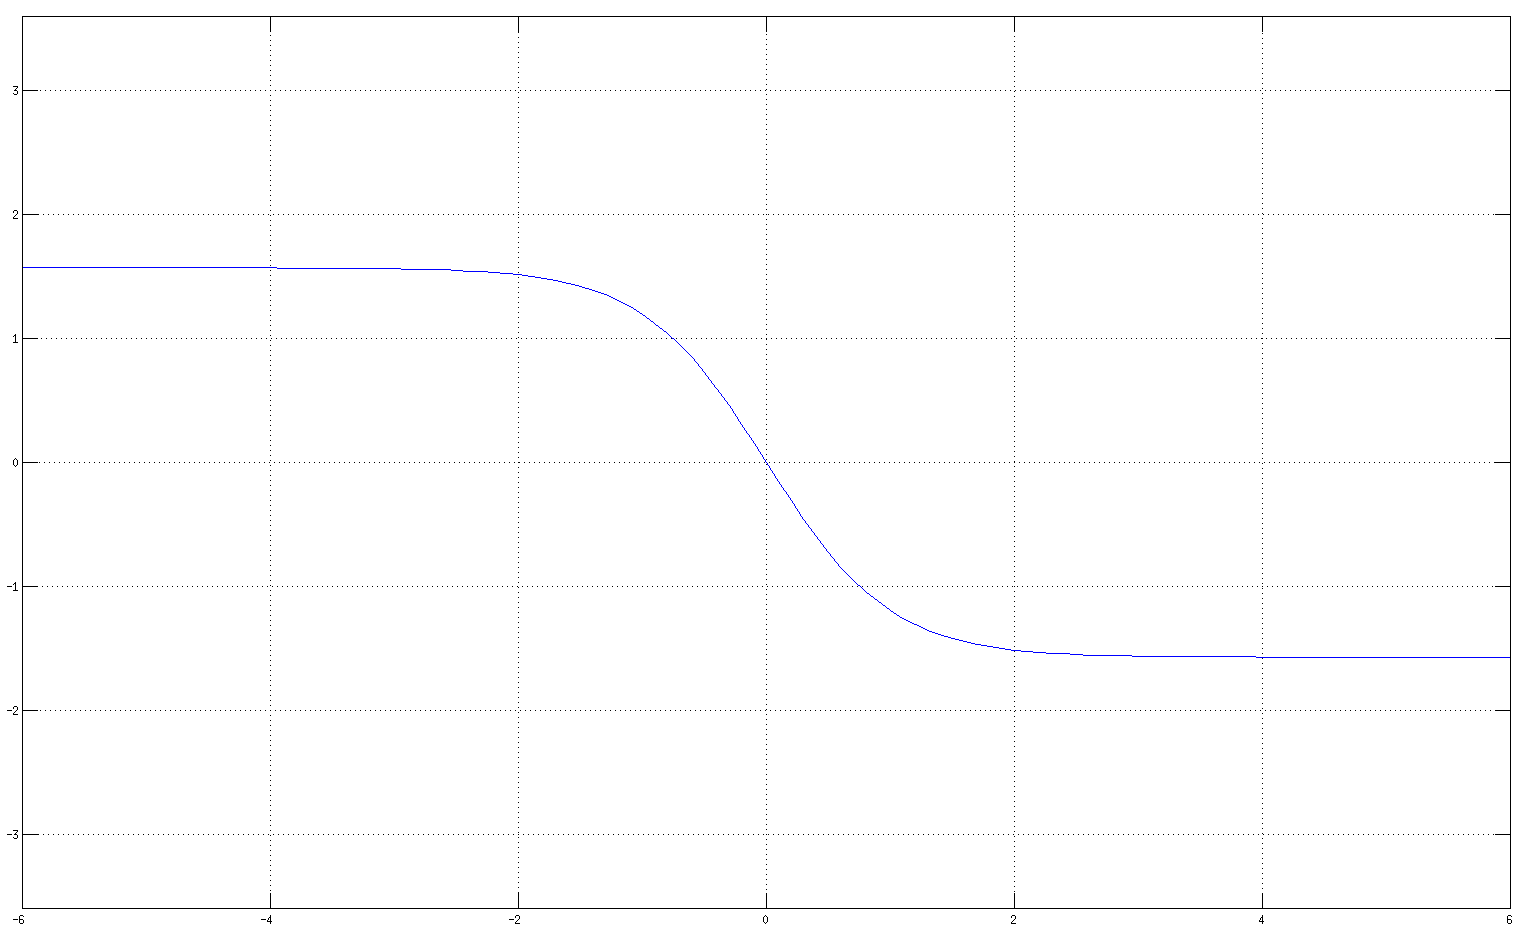
\includegraphics[width=0.5\textwidth]{images/phase_space_tanh_function_graph}\label{fig:phase_space_tanh_function_graph}}
\caption[Sample Phase Space Non-Linear Mapping Functions]{Sample Phase Space Non-Linear Mapping Functions. The horizontal axis in both of these graphs is the lateral offset $d$ and the vertical axis is the desired $\delta\Psi$}
\label{fig:phase_space_sample_function_graphs}
\end{figure}

While the simple piecewise linear function used in this thesis worked well enough, different non-linear mapping functions could be even better. For example, \eqref{eq:phase_space_steering_linear_function} has a pair of discontinuities at the transitions between pieces, easily seen in \autoref{fig:phase_space_linear_function_graph}. These discontinuities did not lead to any observed problems, but could be removed while maintaing the same general shape by using a mapping function based on a sigmoid function (see \todo{add ref http://en.wikipedia.org/wiki/Sigmoid\_function}). See \autoref{fig:phase_space_tanh_function_graph} for an example of a sigmoid function based non-linear mapping that uses the hyperbolic tangent function. The hyperbolic tangent does not have any discontinuties as it approaches its limits and is easily shifted to the interval $\left[-\pi/2,\pi/2\right]$ by multiplying with $\pi/2$, so may be an attractive alternative to the simple piecewise linear function.

\subsection{Lfollow Discussion}\label{subsec:lfollow_discussion_steering}

\begin{comment}
This section details the steering algorithms used by this precision navigation stack

Specifically, the following will be discussed:
\begin{enumerate}
\item Second Order steering (done)
\item Phase Space steering (done)
\item Lfollow for both linear paths and spin in places
	Need to mention the interaction with the PID time constants and such
\item Added a spin in place segment descriptor because of instabilities in the tiny arcs (done)
\end{enumerate}

\end{comment}